\documentclass[12pt]{article}
\usepackage{latexsym}
\usepackage{amssymb,amsmath}
\usepackage[pdftex]{graphicx}
\usepackage{color}
\usepackage{tikz}
\usepackage[margin=0.9in]{geometry}
\usepackage{pifont}
\usepackage{listings}

\begin{document}

\begin{center}
    COMPUTER SCIENCE 20, SPRING 2014 \\
    Week 9 Homework Problems\\
    Trees, Coloring and Growth Rates of Functions \\
    Author: Tawheed Abdul-Raheem 
\end{center}


\smallskip


\begin{enumerate}
    \item 
        In this problem you will prove that a graph $G$ is 2-colorable if and only if $G$ contains no odd-length closed walk.
        \footnote{Adapted from Meyer Problem 11.45}
        \begin{enumerate}
            \item Assume the left side and prove the right side.  Three to five sentences should suffice.
                \textbf{\textit{Solution: }} For any given graph with an odd-length closed walk, the graph cannot be 2-colorable. Given a graph with
                an odd-length, if we label the graph from $p_{i} \text{ to } p_{i+1}$ and assign colors to every other node in our cycle - assign
                {\color{red}RED } to $p_i, p_3, ..., p_{2i+1}$ and the color {\color{blue}BLUE } to $p_2, p_4, ..., p_{2i}$ We notice that when we start
                coloring in a graph with an odd closed walk and alternate the colors, the last first color will be the same as the first color that was
                used. This implies that in a graph with an odd-length closed walk it must be the case we cannot 2-color the graph.
            \item Now assume the right side.  As a first step toward proving the left side, explain why we can focus on a single connected 
                component $H$ of $G$.
                
                \textbf{\textit{Solution :}} We can focus on a single connected component of out graph because that connected compomenet is in one way connected to other parts of our graph. Finding out that a connected component has an odd closed walk tells no matter what we do
            \item As a second step, explain how to 2-color any tree.

                \textbf{\textit{Solution :}} In order to 2-color a tree, you must make sure that two nodes that share a single edge must have a distinct color. Also because this is a tree we are guranteed to not have any closed walk. Alternate the colors of the nodes of the tree. 
            \item Choose any 2-coloring of a spanning tree, $T$, of $H$.  Prove that $H$ is 2-colorable by showing that any edge of $H$ that is 
                \emph{not} in $T$ must also connect different-colored vertices.
                
            \textbf{\textit{Solution :}} Given a spanning tree $H$ in $T$, to prove that $H$ is 2-colorable and that ny edge of H that is not in T must also connect different-colored vertices. We first start by 2-coloring the spanning tree, basically simply alternating our colors. Now lets take that spanning tree out from our tree $T$ and we notice that alternate coloring is also preserved.

        \end{enumerate}


    \item Determine, with justification, the chromatic numbers for the graphs below:

        \begin{enumerate}

            \item \hfill

                \begin{center}
                    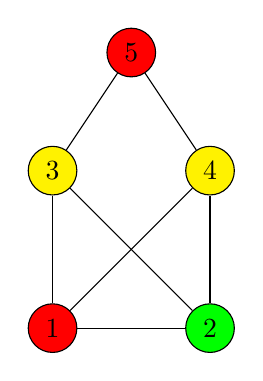
\begin{tikzpicture}
                        \node[fill=red] (1) at (0,0) [shape=circle, draw] {1};
                        \node[fill=green] (2) at (2,0) [shape=circle, draw] {2};
                        \node[fill=yellow] (3) at (0,2) [shape=circle, draw] {3};
                        \node[fill=yellow] (4) at (2,2) [shape=circle, draw] {4};
                        \node[fill=red] (5) at (1,3.5) [shape=circle, draw] {5};

                        \path	[-]	(1)	edge 	(2)
                        edge 	(3)
                        edge 	(4)
                        (2)	edge	(3)
                        edge	(4)
                        (3)	edge	(5)
                        (4)	edge	(5);
                    \end{tikzpicture}
                \end{center}
                The chromatic value $\chi(G) = 3$. The maximum degree of this graph is $3$.The chromatic number of this graph must be less than or equal to $4$. Another important observation
                from this graph is that it cannot be 2-colorable because it has a cycle of odd-length.

            \item \hfill

                \begin{center}
                    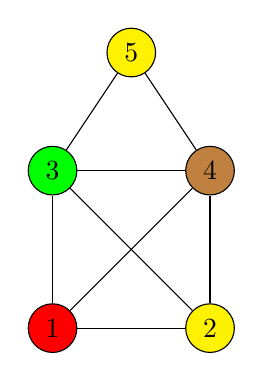
\begin{tikzpicture}
                        \node[fill=red] (1) at (0,0) [shape=circle, draw] {1};
                        \node[fill=yellow] (2) at (2,0) [shape=circle, draw] {2};
                        \node[fill=green] (3) at (0,2) [shape=circle, draw] {3};
                        \node[fill=brown] (4) at (2,2) [shape=circle, draw] {4};
                        \node[fill=yellow] (5) at (1,3.5) [shape=circle, draw] {5};

                        \path	[-]	(1)	edge 	(2)
                        edge 	(3)
                        edge 	(4)
                        (2)	edge	(3)
                        edge	(4)
                        (3)	edge	(4)
                        edge	(5)
                        (4)	edge	(5);
                    \end{tikzpicture}
                \end{center}
                The chromatic value $\chi(G) = 4$. The maximum degree of this graph is $4$. The chromatic number of this graph must be less than or equal to $4$. Another important observation
                from this graph is that it cannot be 2-colorable because it has a cycle of odd-length.

            \item \hfill
                \begin{center}
                    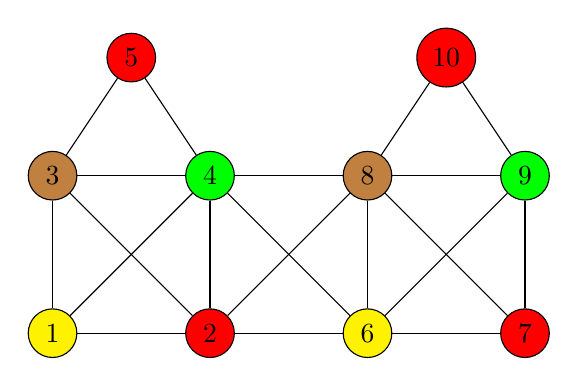
\begin{tikzpicture}
                        \node[fill=yellow] (1) at (0,0) [shape=circle, draw] {1};
                        \node[fill=red] (2) at (2,0) [shape=circle, draw] {2};
                        \node[fill=brown] (3) at (0,2) [shape=circle, draw] {3};
                        \node[fill=green] (4) at (2,2) [shape=circle, draw] {4};
                        \node[fill=red] (5) at (1,3.5) [shape=circle, draw] {5};

                        \node[fill=yellow] (6) at (4,0) [shape=circle, draw] {6};
                        \node[fill=red] (7) at (6,0) [shape=circle, draw] {7};
                        \node[fill=brown] (8) at (4,2) [shape=circle, draw] {8};
                        \node[fill=green] (9) at (6,2) [shape=circle, draw] {9};
                        \node[fill=red] (10) at (5,3.5) [shape=circle, draw] {10};


                        \path	[-]	(1)	edge 	(2)
                        edge 	(3)
                        edge 	(4)
                        (2)	edge	(3)
                        edge	(4)
                        (3)	edge	(4)
                        edge	(5)
                        (4)	edge	(5);

                        \path	[-]	(6)	edge 	(7)
                        edge 	(8)
                        edge 	(9)
                        (7)	edge	(8)
                        edge	(9)
                        (8)	edge	(9)
                        edge	(10)
                        (9)	edge	(10);

                        \path	[-]	(4)	edge	(6)
                        edge	(8)
                        (2)	edge	(6)
                        edge	(8);
                    \end{tikzpicture}
                \end{center}
                The chromatic value $\chi(G) = 4$. The maximum degree of this graph is $6$. The chromatic 
                number of this graph must be less than or equal to $7$. Another important observation
                from this graph is that it cannot be either 2-colorable or 3-colorable because it is a graph that has edeges crossing. 
        \end{enumerate}


    \item In a computer, the values of variables are stored in \textit{registers}, which are small and fast areas of memory on a processor. When compiling source code to machine code, a compiler will try and allocate variables to memories in such a manner as to use the fewest registers possible. Assume that, during the \textit{lifetime of a variable} (from first time it appears in the program to its last use), the compiler keeps that variable in the same register. 

        Cast this problem of allocating registers for variables in terms of graph coloring and give the minimum number of registers needed for the code below. \textit{Hint: in determining edges between vertices, consider the lifetimes of variables.} \footnote{Adapted from Meyer}
        (Take CS 153 to learn more about and implement a fancier version of this process.)

        \begin{verbatim}
            1. input a, b
            2. int c = a - b;
            3. int d = c + a;
            4. int e = d * b;
            5. int f = d * e;
            6. int g = f - 2;
            7. int h = d + 1;
            8. int i = e * d; 
            9. output g, h, i
        \end{verbatim}

        \textbf{\it{Solution: }} \\

        \begin{lstlisting} [
            mathescape,
            columns=fullflexible,
            ]
            1. input $r_1$, $r_2$ 
            2. int $r_3$ = $r_1$ - $r_2$;
            3. int $r_1$ = $r_3$ + $r_1$;
            4. int $r_2$ = $r_1 * r_2$;
            5. int $r_2 = r_1 * r_3$;
            6. int $r_2 = r_2 - 2$;
            7. int $r_4 = r_1 + 1$;
            8. int $r_3 = r_3 * r_1$; 
            9. output $r_2, r_4, r_3$
        \end{lstlisting}


    \item Fill in the following table---check off the box corresponding to functions $f$ and $g$ and relation $\rho$ iff $f(x)$ is $\rho(g(x))$. For example, you would check off the lower-right box if you think that $\sqrt x\sim\log(x)$.

        \begin{center}
            \begin{tabular}{|c|c||c|c|c|c|c|}\hline
                $f(x)$ & $g(x)$ & $O$ & $o$ & $\Omega$ & $\Theta$ & $\sim$\\\hline
                $x$ & $x + 100$ & & & & {\checkmark}& {\checkmark}\\\hline
                $(0.1)^x$ & $1$ & {\checkmark}& & & & \\\hline
                $2^x$ & $3^x$ & {\checkmark}& {\checkmark}& {\checkmark}& & \\\hline
                $\log(x)$ & $\log(x^2)$ & & {\checkmark}& & & \\\hline
                $1/x$ & $1/\sqrt{x}$ & & {\checkmark}& & & \\\hline
                $\sqrt x$ & $\log(x)$ & & {\checkmark}& &  & \\\hline
            \end{tabular}
        \end{center}

    \item Show that $O$ is a transitive relation.  That is, show that if $h$ is $O(g)$ and $g$ is $O(f)$, then $h$ is $O(f)$.\\
        \textbf{\textit{Solution: }} We want to prove that 
        \[ \text{ if } h \rightarrow  O(g) \text{ and } g \rightarrow O(f) \text{ then } h \rightarrow O(f) \]
    To prove the above we assume that $g(x) $ is $O(f(y))$ there exists some $ x, y$ in our function. From this we can see that because $x$ has a relationship from $h$ and also $x$ has a mapping to $y$. Then it must be the case that because of the relationship that $x$ and $h$ has it implies that $h$ also maps to $y$
\end{enumerate}
\end{document}
